% \section{Experiments}
% In this section we benchmark our algorithm for dropping labels from a dataset.

% \subsection{Setup}
% We consider two examples, one 
% The goal of our experiments is to evaluate the empirical performance of the Chaining Sampling Algorithm (CSA). In particular, we aim to:
% \begin{itemize}
%     \item Evaluate CSA on synthetic and real data. 
%     \item Compare performance against competing algorithms 
%     \item (potential)
%     \item Measure label efficiency.
%     \item Evaluate regression performance via $\|Xw' - y\|_2^2$.
%     \item Verify theoretical approximation $(1 + d/N)$ in practice.
    
    
% \end{itemize}

% \subsection{Algorithms Comparison}

% \begin{itemize}
%     \item \textbf{Chaining Sampling Algorithm}
%     \item \textbf{.}
% \end{itemize}

% Each algorithm will be evaluated using the following:
% \begin{itemize}
%     \item Approximation ratio:
%     \[
%     \frac{\|Xw' - y\|_2^2}{\|Xw^* - y\|_2^2}
%     \]
%     \item Label complexity
%     \item Runtime
% \end{itemize}


% \subsection{Synthetic Dataset}

% \subsubsection{Data Generation}

% \begin{itemize}
%     \item.
% \end{itemize}

% \subsubsection{Experimental Setup}

% \begin{itemize}
%     \item .
% \end{itemize}


% \subsubsection{Evaluation}
% On synthetic datasets we aim to evaluate:
% \begin{itemize}
%     \item Whether the approximation ratio matches the theoretical bound $1 + O(d/N)$.
%     \item How many data points can be removed before performance degrades.
% \end{itemize}

% \subsection{Real Dataset}

% \subsubsection{Dataset Description}

% \begin{itemize}
%     \item .
% \end{itemize}

% \subsubsection{Experimental Setup}

% \begin{itemize}
%     \item .
% \end{itemize}


% \subsubsection{Evaluation}

% \begin{itemize}
%     \item Whether the approximation ratio matches the theoretical bound $1 + O(d/N)$.
%     \item How many data points can be removed before performance degrades.
% \end{itemize}

% \subsection{Results and Analysis}

% \subsubsection{Potential things to evaluate in analysis}

% \subsubsection{Error vs. Label Complexity}

% \subsubsection{Approximation Ratio}

% \subsubsection{Assumption Validation}

% \subsubsection{Discussion}
% \begin{itemize}
%     \item .
% \end{itemize}

% \subsection{Summary of Findings}
% Our experiments highlight:
% \begin{itemize}
%     \item .
% \end{itemize}

\section{Experiments}
In this section, we evaluate the Chaining Sampling Algorithm (CSA) on both synthetic and real datasets, with the goal of approximating regression weights using fewer observed labels.

\subsection{Setup}
The primary objective is to determine how many labels we can safely "discard" while maintaining a predictive error close to the full-dataset solution. We evaluate the performance across varying dimensions $d$ and sample sizes $N$. In particular, benchmark CSA against some baseline sampling methods and validate the approximation ratio (\(1 + d/N\)).

We consider the synthetic and real setting in our experiments.
In the synthetic setting we create two examples using scikit-learn parametric datasets \citep{scikit-learn}. In the first example we create a randomized regression problem with \(d=10\) with \(5\) informative features sampled with Gaussian noise with standard deviation \(0.002\). In the second example we use the classical two moons dataset for classification with standard deviation noise of \(0.005\). In both examples we use \(N=1000\) samples.
In the real-world datasets we consider the wine quality dataset from \citet{wine_quality_186} and the concrete compressive strength dataset from \citet{concrete_compressive_strength_165}.
We measure the relationship of the approximation ratio to the label budget. In each example we remove up-to 60\% of the labels to produce our experiments. We further just do naive linear regression without further feature engineering.

\subsection{Results}
We discuss what assumptions are broken by our datasets that make CSA fail.

In Figure~\ref{fig:naive}, we initialize a dataset with $N = 1000$ samples in $d = 10$ dimensions, along with randomly generated labels. Applying CSA, we are able to remove up to 50\% of the labels while remaining within the target approximation bound.

As shown in Figure~\ref{fig:naive}, the approximation error decreases steadily as the label budget increases, and remains consistently below the theoretical threshold of $d/N$. Notably, CSA maintains a stable approximation ratio even after discarding a significant portion of the dataset. This result indicates that many data points contribute little to the overall regression fit. The smooth decay in error suggests that the CSA algorithm effectively targets uninformative samples in the dataset, leading to a stable decrease in error over a large range of the label budget. 

These results are consistent with the theoretical guarantees, as the observed approximation error remains stable and does not exhibit exponential decay that might be expected from iterative data removal. This result provides empirical support for the effectiveness of the CSA algorithm.

To further explore this behavior, we consider additional synthetic benchmarks. In Figure~\ref{fig:syn_moons}, we evaluate CSA on the two-moons dataset. In this setting, CSA is only able to remove approximately 10\% of the labels before reaching the target approximation bound, representing a substantial deviation from the conjectured 50\% removal. This suggests that when the data contains strong non-linearity, a larger fraction of samples becomes essential for preserving an accurate fit.

In contrast, Figure~\ref{fig:syn_regression} shows results on a synthetic regression benchmark with less restrictive structure and more uniform contributions from each instance. CSA is able to remove close to 50\% of the labels while remaining within the target approximation bound, closely aligning with the conjectured behavior observed in earlier experiments.

This motivates further investigation into more realistic settings, where data distributions may be more structured or exhibit complex dependencies. Evaluating CSA on real data will reveal more about capabilities and limitations of CSA in practice.

We evaluate CSA on several benchmark regression datasets commonly used in empirical studies. Specifically, we consider the wine quality datasets, considering both the red and white wine variants, and the concrete compressive strength dataset. Unlike the synthetic setting, these datasets reflect the nontrivial interactions among features that are characteristic of real-world data, which violate the assumptions under which CSA performs optimally.

For each dataset, we apply CSA under the same experimental protocol as in the synthetic case, varying the label budget and measuring the resulting approximation error relative to the full dataset solution. Figure~\ref{fig:real_data} summarizes the performance of CSA across different label budgets for each dataset.

Applying CSA to both the red and white wine quality datasets, we observe in Figure~\ref{fig:real_rw} and \ref{fig:real_ww}, we are able to remove up to approximately 30\% of the labels while remaining within the target approximation bound. 

For the concrete compressive strength dataset, we observe in Figure~\ref{fig:real_concrete} that CSA is able to remove a larger percentage of the labels before reaching the target approximation bound, up to nearly 50\%.

These results highlight how deviations from idealized assumptions impact the performance of CSA. In particular, the presence of real world data, which exhibits complex feature interactions and variable sample importance, limits CSA’s ability to reliably identify and discard uninformative points, leading to degraded approximation quality. 

Overall, the experiments across both synthetic and real-world datasets reveal a mixed alignment with the conjectured behavior of CSA. In some settings, particularly those where the data exhibits a uniform sample importance, CSA achieves performance close to the theoretical expectation, resulting in near 50\% label removal. However, in cases where data exhibits more structure or non-linearity, in both synthetic and real-world data, CSA deviates from the conjecture and exhibits significantly reduced label removal capacity.



\begin{figure}
    \centering
    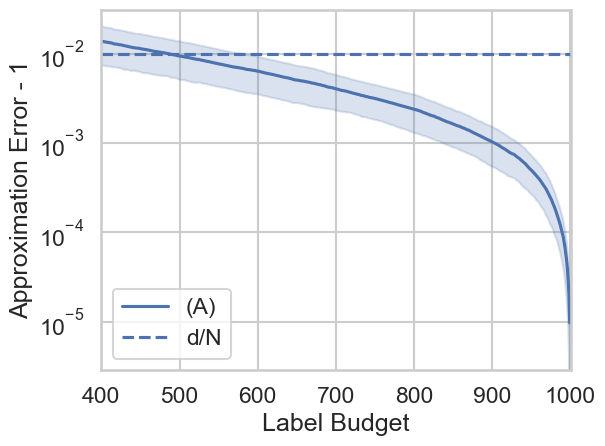
\includegraphics[width=0.5\linewidth]{figures/naive_budget.png}
    \caption{CSA can easily have removed points if noise is random rather than adversarial. (A) is CSA. The shaded region is within 1-standard deviation.}
    \label{fig:naive}
\end{figure}
\begin{figure}
  \centering
  \subfloat[Two moons\label{fig:syn_moons}]{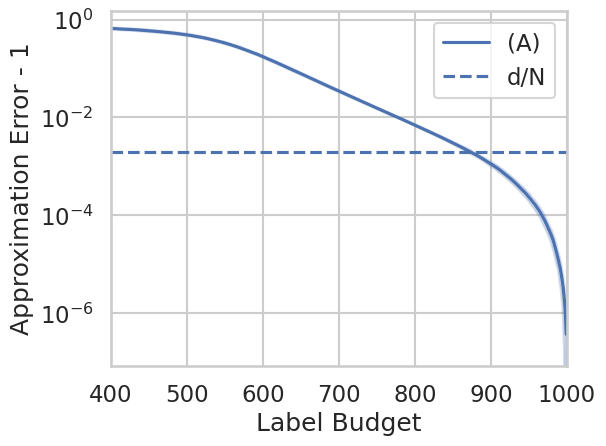
\includegraphics[width=0.4\textwidth]{figures/moons.png}}\qquad
  \subfloat[Synthetic Regression\label{fig:syn_regression}]{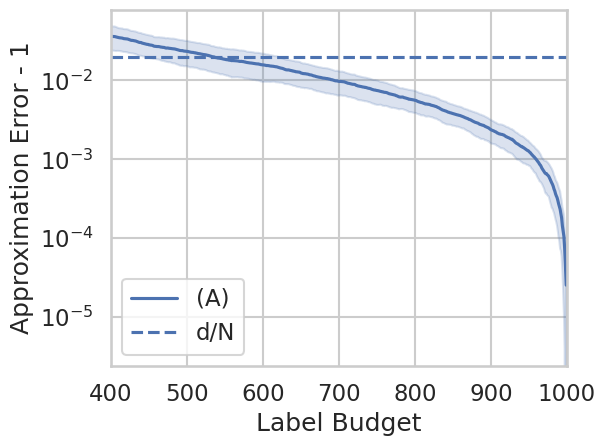
\includegraphics[width=0.4\textwidth]{figures/synthetic_regression.png}}
\caption{Synthetic datasets. In \ref{fig:syn_moons}, we only remove roughly 10\% of the rows before we reach the approximation ratio, this is likely due to being a classification problem. In \ref{fig:syn_regression}, we can remove nearly 50\% of the labels in the dataset matching our conjecture.}
\label{fig:synthetic_dataset}
\end{figure}

\begin{figure}
  \centering
  \subfloat[Red Wine Quality\label{fig:real_rw}]{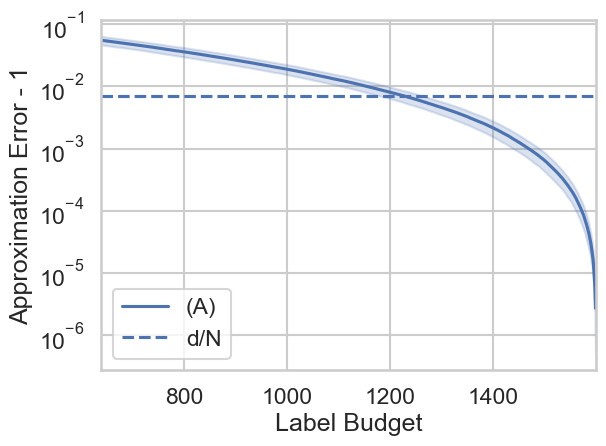
\includegraphics[width=0.3\textwidth]{figures/WineQualityRed_Fixed.png}}\qquad
  \subfloat[White Wine Quality\label{fig:real_ww}]{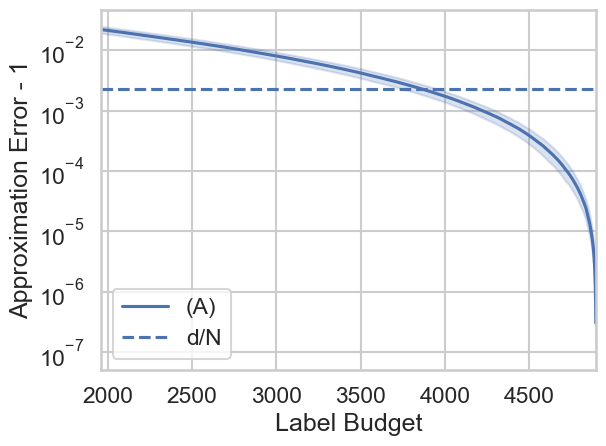
\includegraphics[width=0.3\textwidth]{figures/WineQualityWhite_Fixed.png}}\qquad
  \subfloat[Concrete Strength\label{fig:real_concrete}]{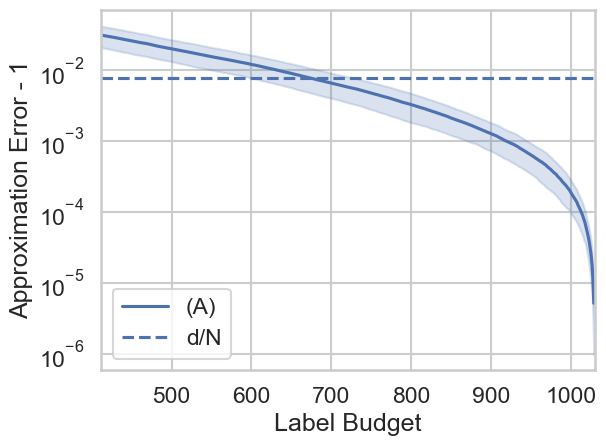
\includegraphics[width=0.3\textwidth]{figures/Concrete_Fixed.png}}
\caption{We remove roughly 30\% of the labels before our approximation ratio is achieved in the wine datasets. The concrete dataset removes roughly 50\%.}
\label{fig:real_data}
\end{figure}